\section{Parallel tempering}
\label{sec:PT}
Pigeons.jl provides an implementation of distributed parallel tempering (PT) described 
in \cite{syed2021nrpt}, which we outline in Algorithm~\ref{alg:distributed_PT}.
This section gives both a brief overview of PT and some details of 
its distributed implementation.

In this section we assume a basic understanding of 
Markov chain Monte Carlo (MCMC) methods.
For readers unfamiliar with MCMC, it is important to know that 
it is a method to obtain approximate samples from a distribution. 
However, with traditional 
MCMC methods, the samples may be heavily correlated instead of independent 
and may fail to sufficiently explore the 
full space of the distribution (see \cref{fig:bimodal}); 
PT is a method that aims to address these issues.
For a more in-depth review of PT, we refer readers to \cite{surjanovic2022vpt}.


\subsection{Overview of PT}
Suppose that we would like to estimate integrals involving $\pi$, such as 
$\int f(x) \pi(x) \, \dee x$. 
These integrals may be multivariate and even include combinations of 
continuous and discrete variables (where sums replace integrals in the discrete 
case).
One method is to obtain samples from $\pi$ to approximate such integrals.
Often, the distribution 
$\pi$ can be challenging for traditional MCMC methods---such 
as Metropolis-Hastings, slice sampling, and Hamiltonian Monte Carlo---
because of its structure.
For example, in a bimodal example such as the one illustrated in 
Figure~\ref{fig:bimodal},
traditional methods might remain in one of the two modes for an extremely 
long period of time.

\begin{figure}[t]
    \centering
    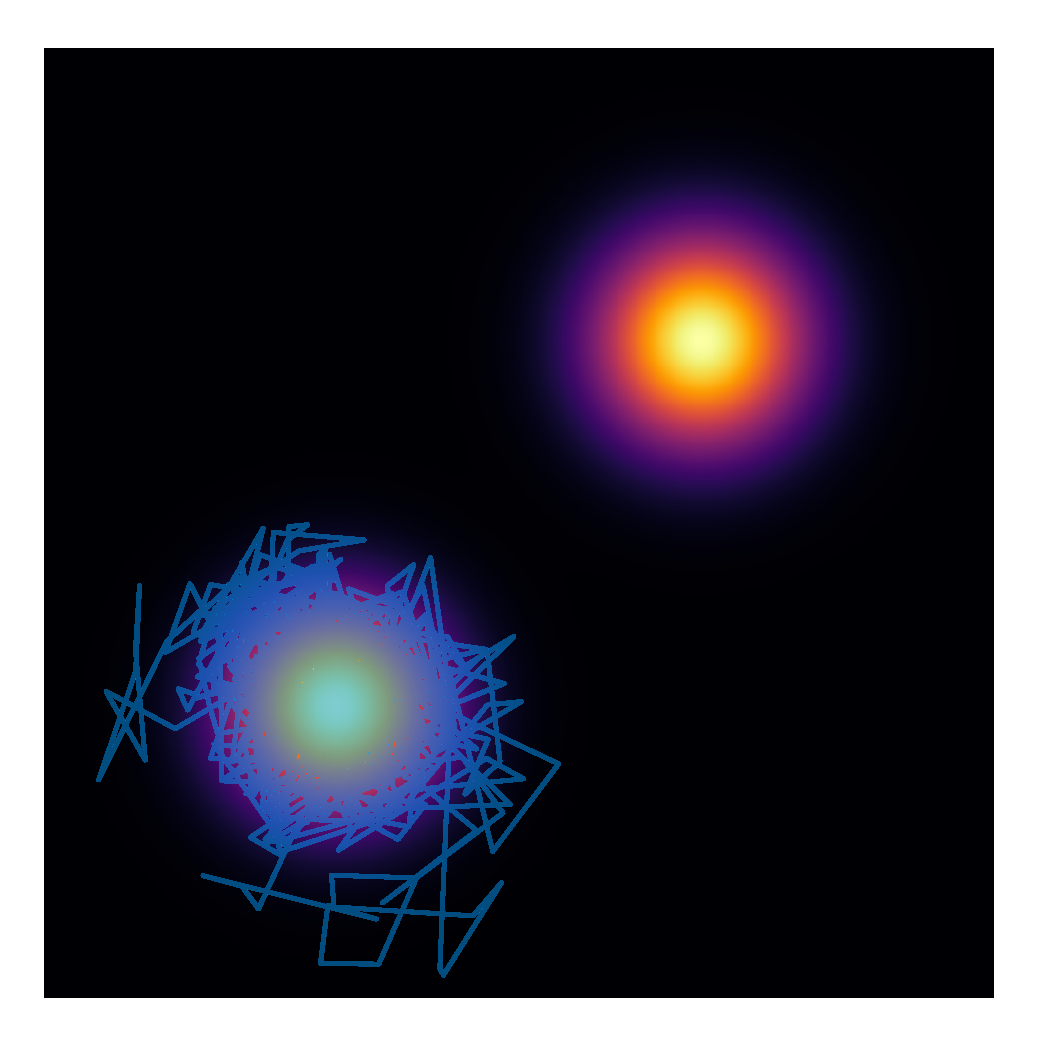
\includegraphics[width=0.3\textwidth]{../img/bimodal.pdf}
    \caption{A simple bimodal distribution from which traditional 
    MCMC methods may struggle to obtain samples. Blue lines display output 
    from 1,000 iterations of a Metropolis-Hastings random walk MCMC algorithm.
    The sampler in this figure is visibly trapped in one of the two modes.}
    \label{fig:bimodal}
\end{figure}


To resolve this issue, PT constructs a sequence of $N$ distributions,  
$\pi_1, \pi_2, \ldots, \pi_N$, where $\pi_N$ is usually equal to $\pi$.
The distributions are chosen so that it is easy to obtain samples from $\pi_1$
with the sampling difficulty increasing as one approches $\pi_N$. An example 
of such a sequence of distributions, referred to as an \textit{annealing path},
is shown in Figure~\ref{fig:path}.

\begin{figure*}[t]
    \centering
    \begin{minipage}{0.15\textwidth}
      \centering
      
\includegraphics[width=\textwidth]{../img/heatmap_path_1.pdf}
      \caption*{$\pi_1$}
    \end{minipage}
    \begin{minipage}{0.15\textwidth}
      \centering
      
\includegraphics[width=\textwidth]{../img/heatmap_path_2.pdf}
      \caption*{$\pi_2$}
    \end{minipage}
    \begin{minipage}{0.15\textwidth}
      \centering
      
\includegraphics[width=\textwidth]{../img/heatmap_path_3.pdf}
      \caption*{$\pi_3$}
    \end{minipage}
    \begin{minipage}{0.15\textwidth}
      \centering
      
\includegraphics[width=\textwidth]{../img/heatmap_path_4.pdf}
      \caption*{$\pi_4$}
    \end{minipage}
    \begin{minipage}{0.15\textwidth}
      \centering
      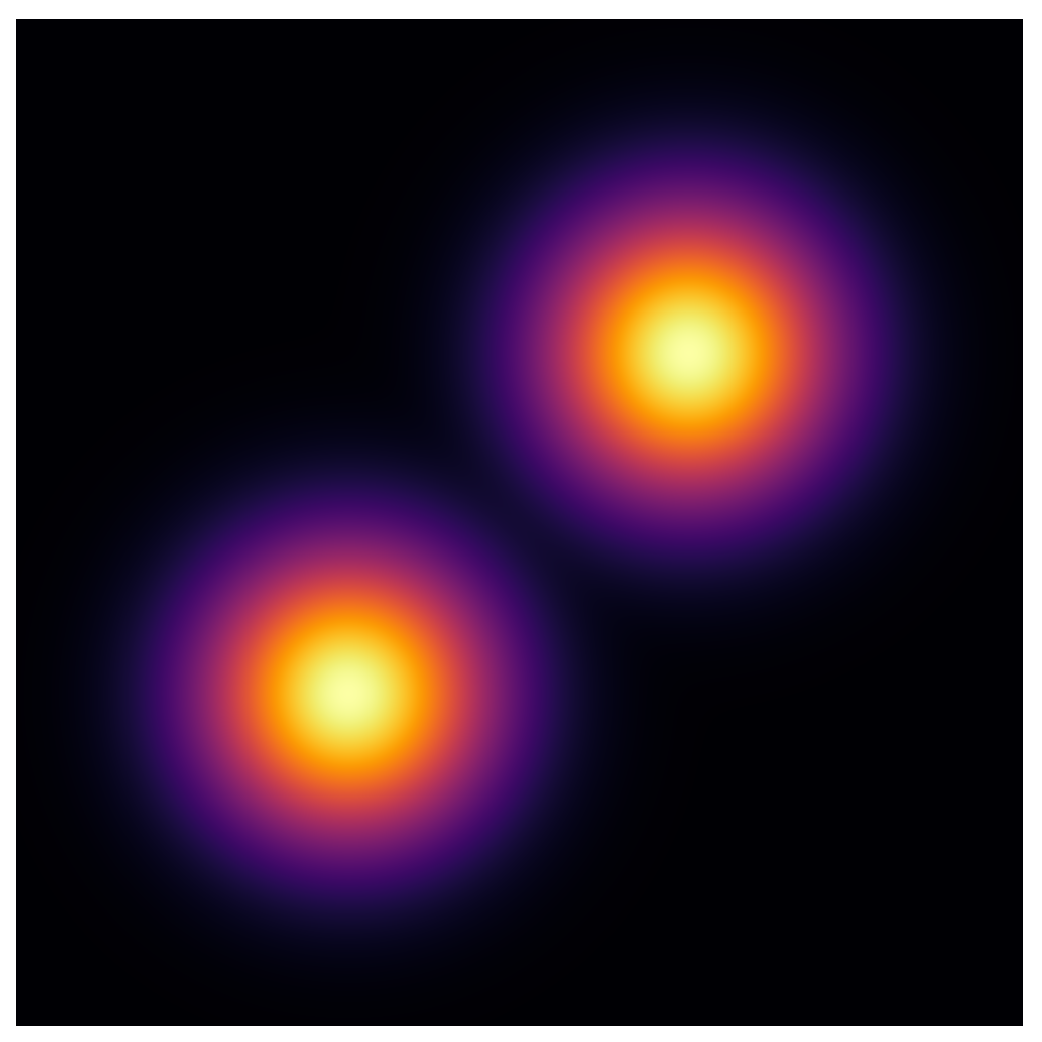
\includegraphics[width=\textwidth]{../img/heatmap_path_5.pdf}
      \caption*{$\pi_5$}
    \end{minipage}
    \begin{minipage}{0.15\textwidth}
      \centering
      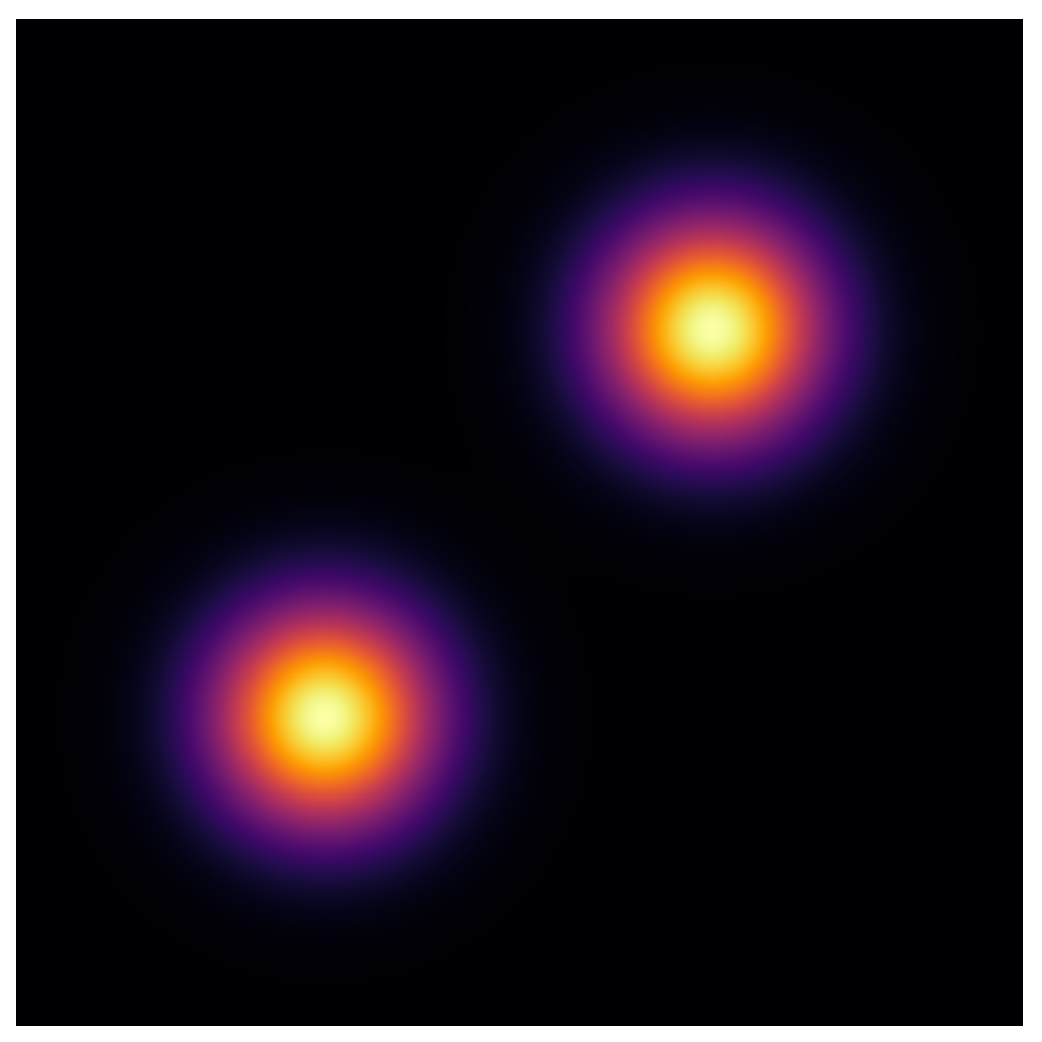
\includegraphics[width=\textwidth]{../img/heatmap_path_6.pdf}
      \caption*{$\pi_6$}
    \end{minipage}
    \caption{Heatmaps of six distributions lying on an annealing path 
    from a unimodal reference distribution  
    $\pi_1$, from which it is straightforward to obtain samples, and ending at 
    $\pi_N$, which is in this case the bimodal distribution from 
    Figure~\ref{fig:bimodal}. (Note that in this case the colours between the heatmaps 
    are not directly comparable because the densities of intermediate distributions 
    are not normalized.)}
    \label{fig:path}
\end{figure*}


We now turn to explain how this path of distributions can be used to enhance 
sampling from the target distribution, $\pi$. 
PT operates by first obtaining samples from each distribution on the path in parallel 
(referred to as an \textit{exploration phase}). 
Then, samples between adjacent distributions are swapped (referred to as 
a \textit{communication phase}). The communication phase in PT is crucial: it allows 
for the discovery of new regions of the space of the target distribution such as 
the top-right mode of the distribution presented in Figure~\ref{fig:bimodal}. 


\subsection{Local exploration and communication}
A central data structure in Pigeons is the \texttt{Replica}, a Julia struct 
that we will often refer to in the remainder of this section. 
A single \texttt{Replica} stores a \texttt{state} variable and a \texttt{chain} 
integer, among other entries. 
At the beginning of PT, $N$ \texttt{Replicas} are created, 
one for each distribution on the annealing path, and 
the chain entries in the $N$ replicas are initialized at $1,2,\ldots,N$, respectively. 
For a given \texttt{Replica}, if the \texttt{chain} number is $i$ and the \texttt{state}
is $x$, then this means that the sample corresponding to the $i$-th distribution in 
the sequence $\pi_1, \ldots, \pi_N$ is currently at location $x$.  

 
In the local exploration phase,
each \texttt{Replica}'s state is modified using an MCMC move targeting $\pi_i$,
where $i$ is given by \texttt{Replica.chain}.
The MCMC move can either modify \texttt{Replica.state} in-place, or modify the 
\texttt{Replica}'s \texttt{state} field. 
This operation is indicated by the \texttt{local\_exploration} function in 
\cref{alg:distributed_PT}.

 
In the communication phase, PT proposes swaps between pairs of replicas. 
In principle, there are two equivalent ways to do a swap.
In the first implementation, the \texttt{Replica}s 
could exchange their \texttt{state} fields.
Alternatively, they could exchange their \texttt{chain} fields.
Because we provide distributed implementations, we use the latter as it ensures that 
the amount of data that needs to be exchanged between two machines during a swap 
can be made very small (two floating point numbers), resuling in 
an exchange of $O(N)$ messages of size $O(1)$. 
Note that this cost does not vary with the dimensionality of the state space, 
in contrast to the first implementation that would transmit 
$O(N)$ messages of size $O(d)$, where $d$ is the dimension of the state space,
incurring a potentially very high communication cost for large values of $d$.


\subsection{Distributed implementation}
A distributed implementation of PT is shown in \cref{alg:distributed_PT}
and we describe the details of the implementation below.
For pedagogy, we first present the algorithm in the special case where the number of machines available 
is equal to the number of \texttt{Replica}s and distributions, $N$. 
However, Pigeons also allows for the more general case where the number of 
machines is not necessarily equal to $N$.
We outline how Pigeons achieves this in \cref{sec:relax}.


\subsubsection{Distributed mapping from chains to machines}
\label{sec:permuted_dist_array}
Recall that our theoretical $O(1)$ message size for communication between two machines 
is achieved by exchanging \texttt{chain} indices between \texttt{Replica}s 
instead of their \texttt{state}s. 
However, in order to achieve this low cost, a specialized distributed data structure is 
needed to maintain a mapping from chain indices to machine identifiers. 
To motivate it, we start with an illustrative example. 
Suppose we have $N=4$ distributions, chains, replicas, and machines, and that 
machine 1 is exploring chain 2 while machine 4 is exploring chain 3.
At one point, the \texttt{Replica} at \texttt{chain} 2 (machine 1) might need to exchange
\texttt{chain} indices with the \texttt{Replica} that has \texttt{chain} index 3 (machine 4). 
However, a priori it is not clear how machine 1 should know that it should communicate 
with machine 4 because it has no knowledge about the chain indices on the other machines.

 
To resolve this issue, we introduce a special data structure called a 
\texttt{PermutedDistributedArray}. In the case where the number of replicas is 
equal to the number of available machines, the construction is quite simple
and effectively results in each machine storing one additional integer. 
Considering the same example above, the solution to the problem is to have
machine 1 (\texttt{chain} 2 wanting to communicate with \texttt{chain} 3) 
communicate with \textit{machine} 3. 
Machine 3 stores in its \texttt{dist\_array} variable of type 
\texttt{PermutedDistributedArray} the value 4, which is the machine number that 
stores \texttt{chain} 3. By updating these \texttt{PermutedDistributedArray} 
variables at each communication step, we can ensure that each machine $j$ is aware 
of which machine number currently stores \texttt{chain} $j$. 
Therefore, the machines act as keys in a dictionary for the communication 
permutations.
An illustration of communication between four machines is provided in 
\cref{fig:index_process}.
We note that with a \texttt{PermutedDistributedArray} we make special assumptions 
on how we access and write to the array elements. 
Several MPI processes cooperate, with each machine storing 
data for a slice of this distributed array, and at each time 
step an index of the array is manipulated by exactly one machine. 
Thanks to this, we do not need to resort to global MPI synchronization steps. 

\begin{figure*}[t] 
  \centering 
  \begin{minipage}{0.48\textwidth}
    \centering
    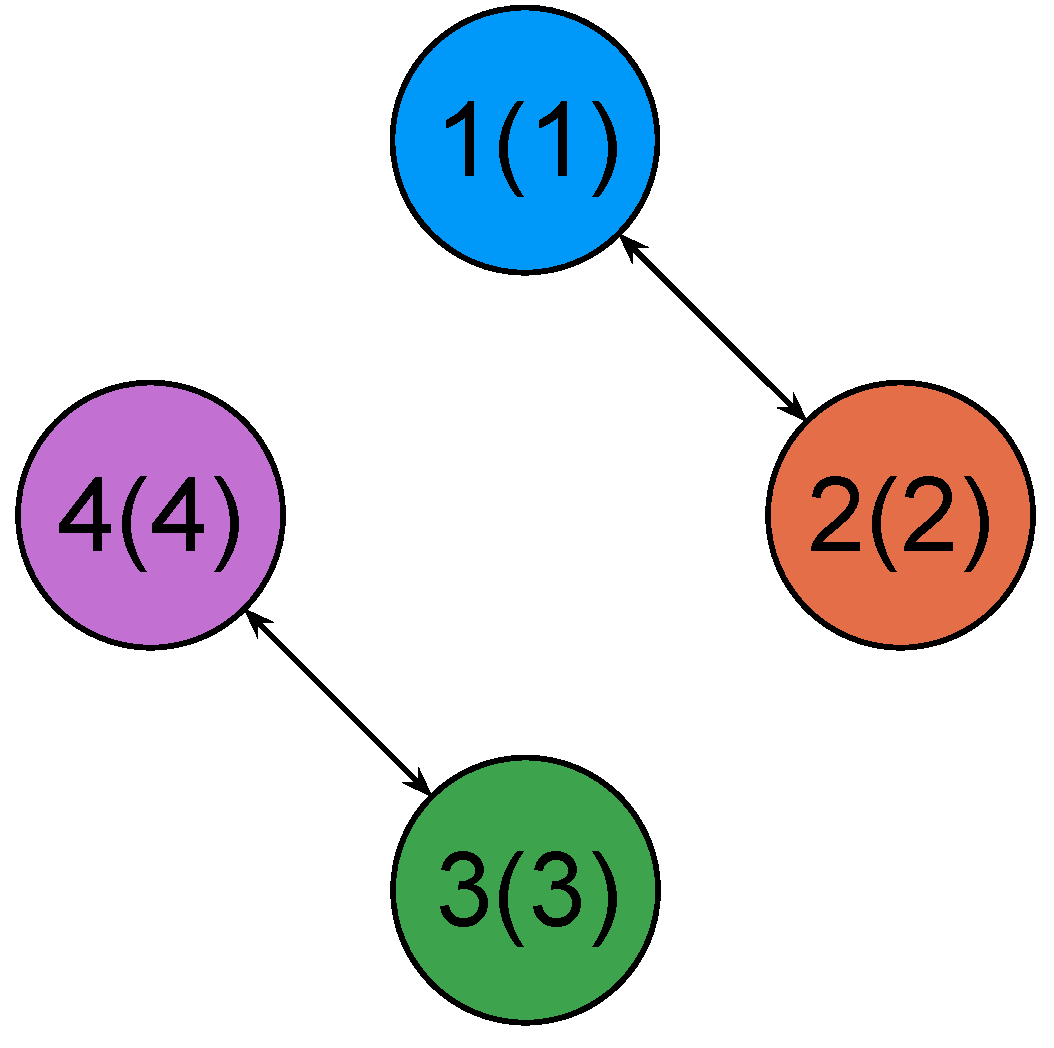
\includegraphics[width=0.39\textwidth]{../img/Communication_1_v3.pdf}
    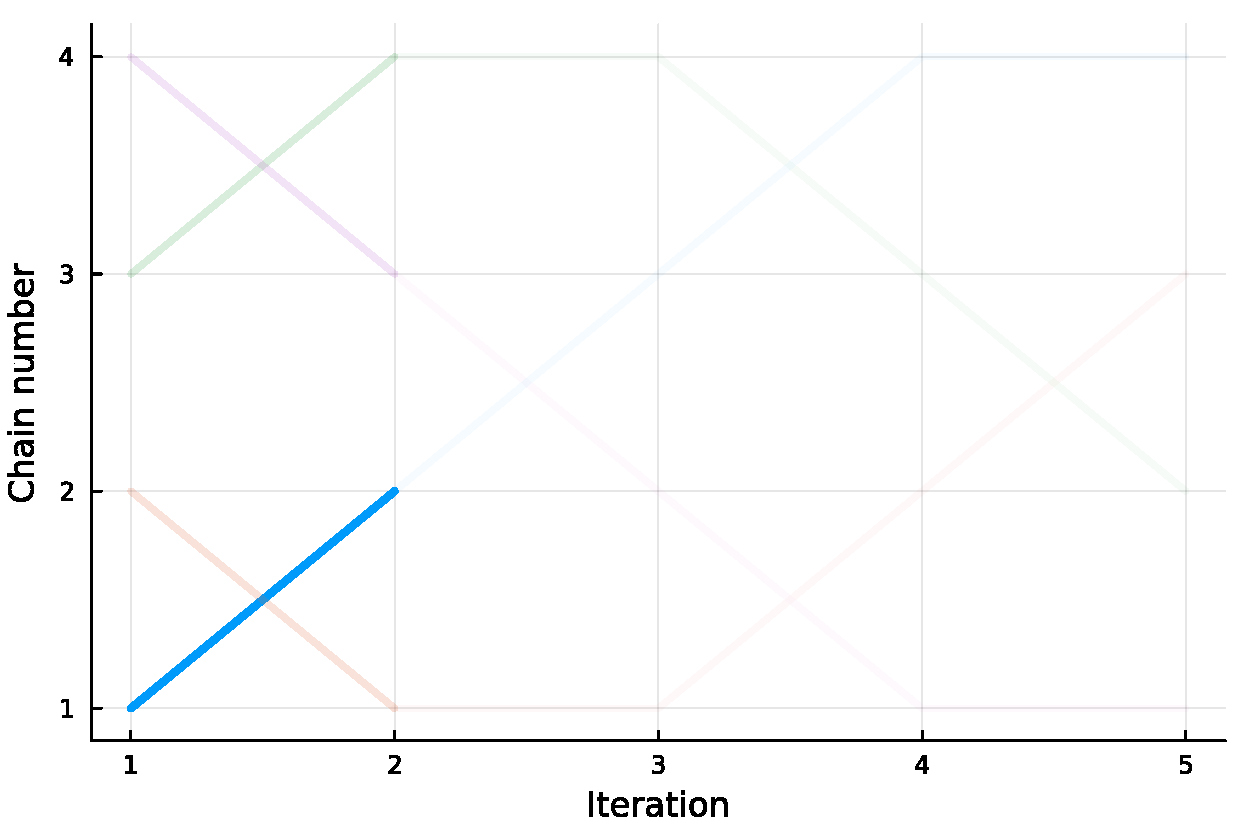
\includegraphics[width=0.59\textwidth]{../img/index_process_1.pdf}
  \end{minipage}
  \begin{minipage}{0.48\textwidth}
    \centering
    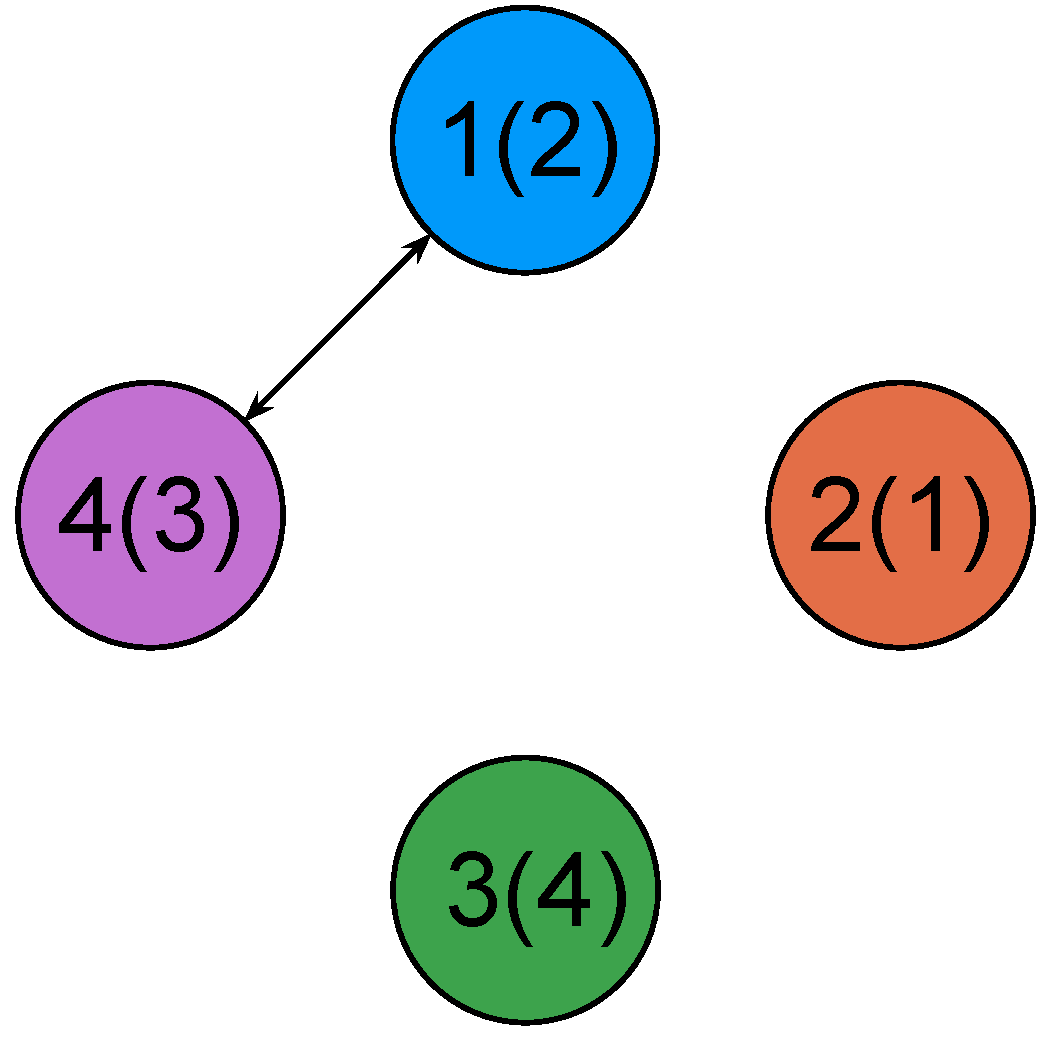
\includegraphics[width=0.39\textwidth]{../img/Communication_2_v3.pdf}
    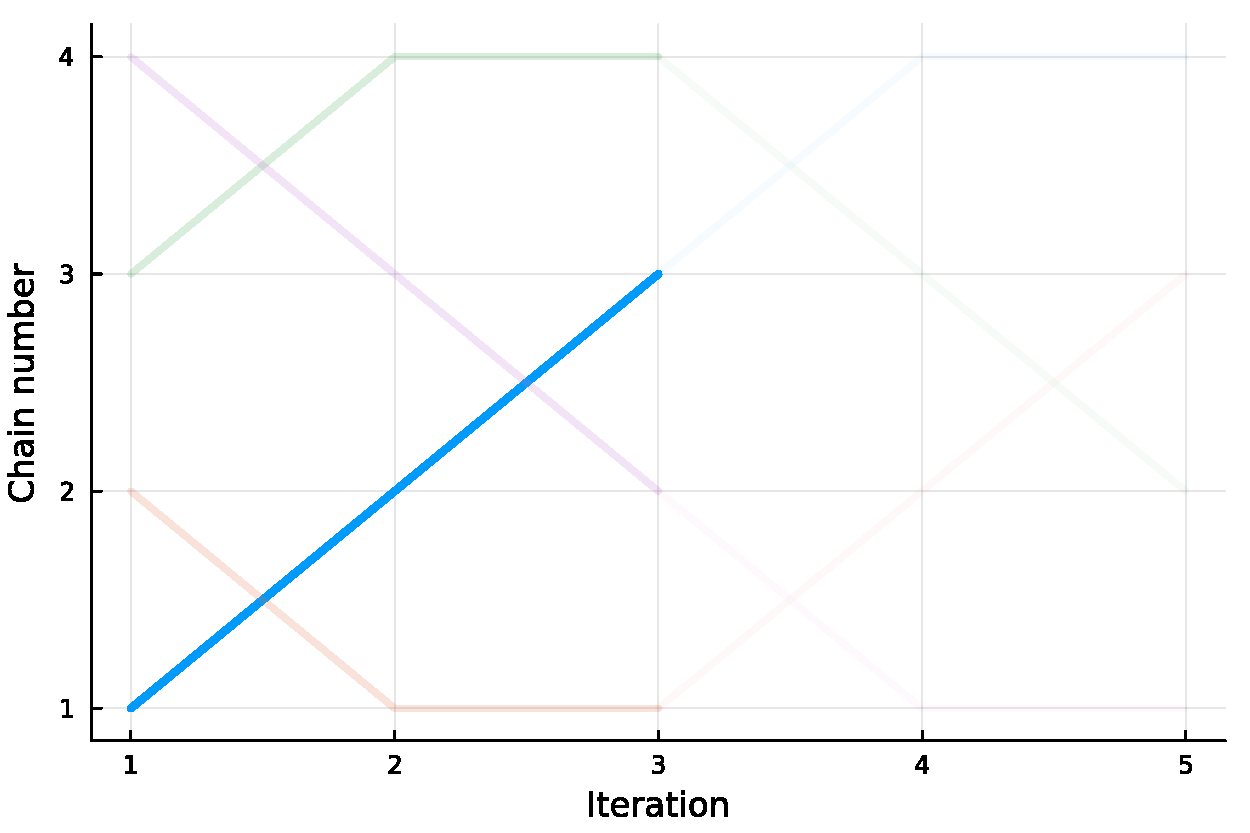
\includegraphics[width=0.59\textwidth]{../img/index_process_2.pdf}
  \end{minipage}
  \begin{minipage}{0.48\textwidth}
    \centering
    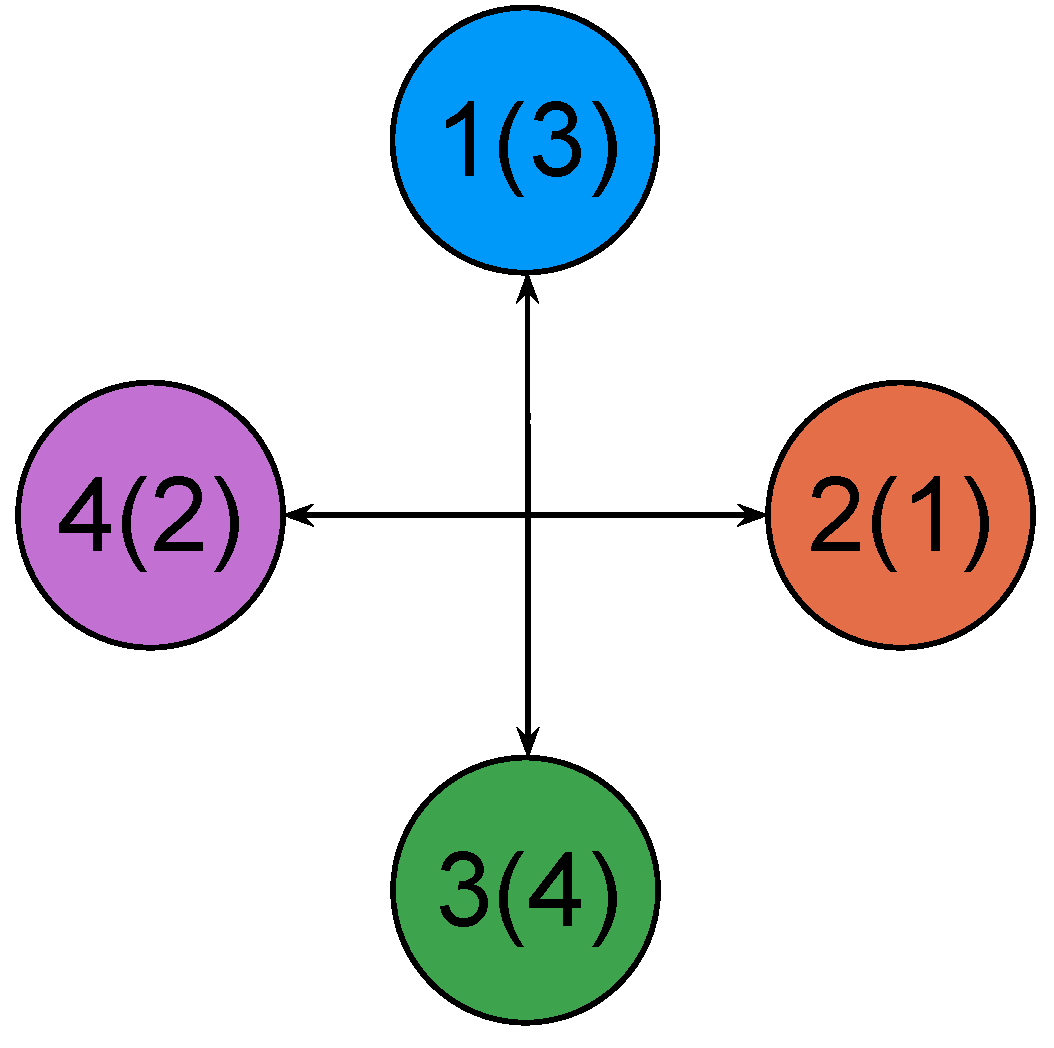
\includegraphics[width=0.39\textwidth]{../img/Communication_3_v3.pdf}
    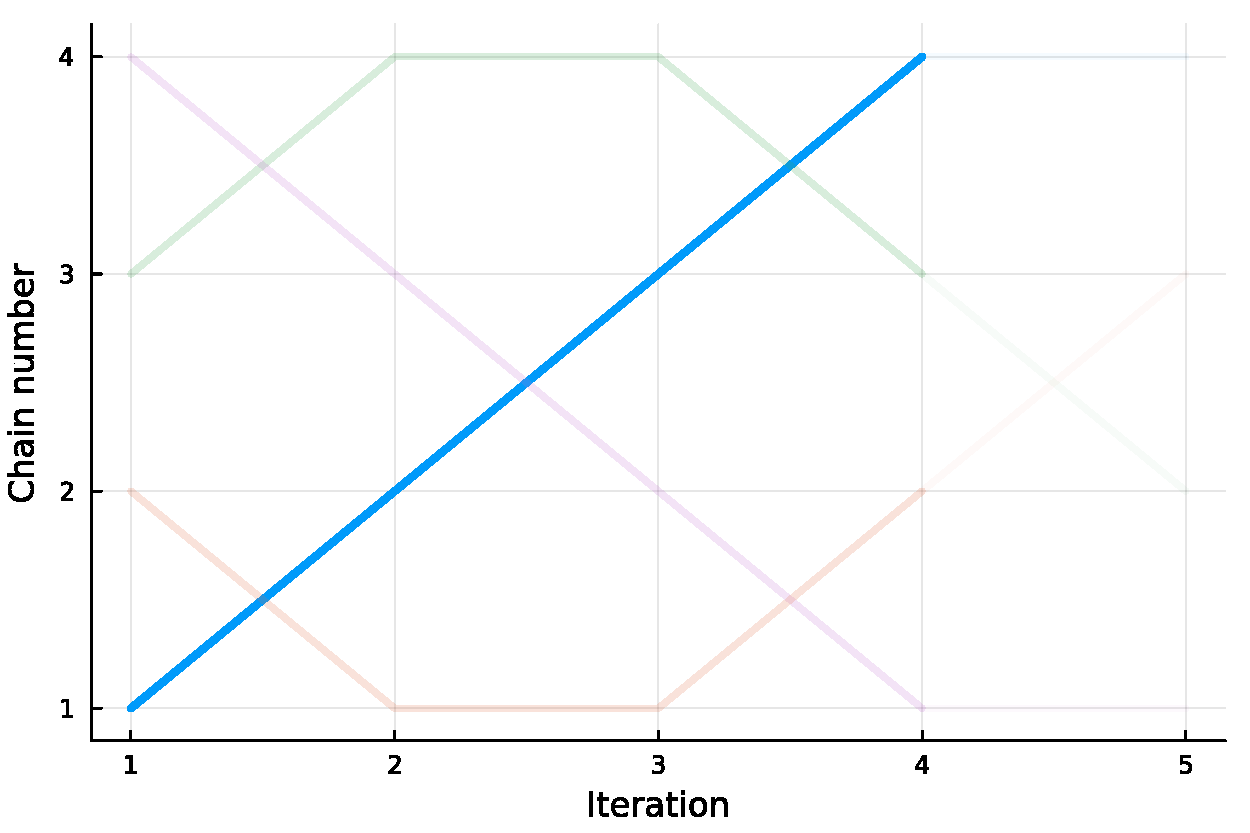
\includegraphics[width=0.59\textwidth]{../img/index_process_3.pdf}
  \end{minipage}
  \begin{minipage}{0.48\textwidth}
    \centering
    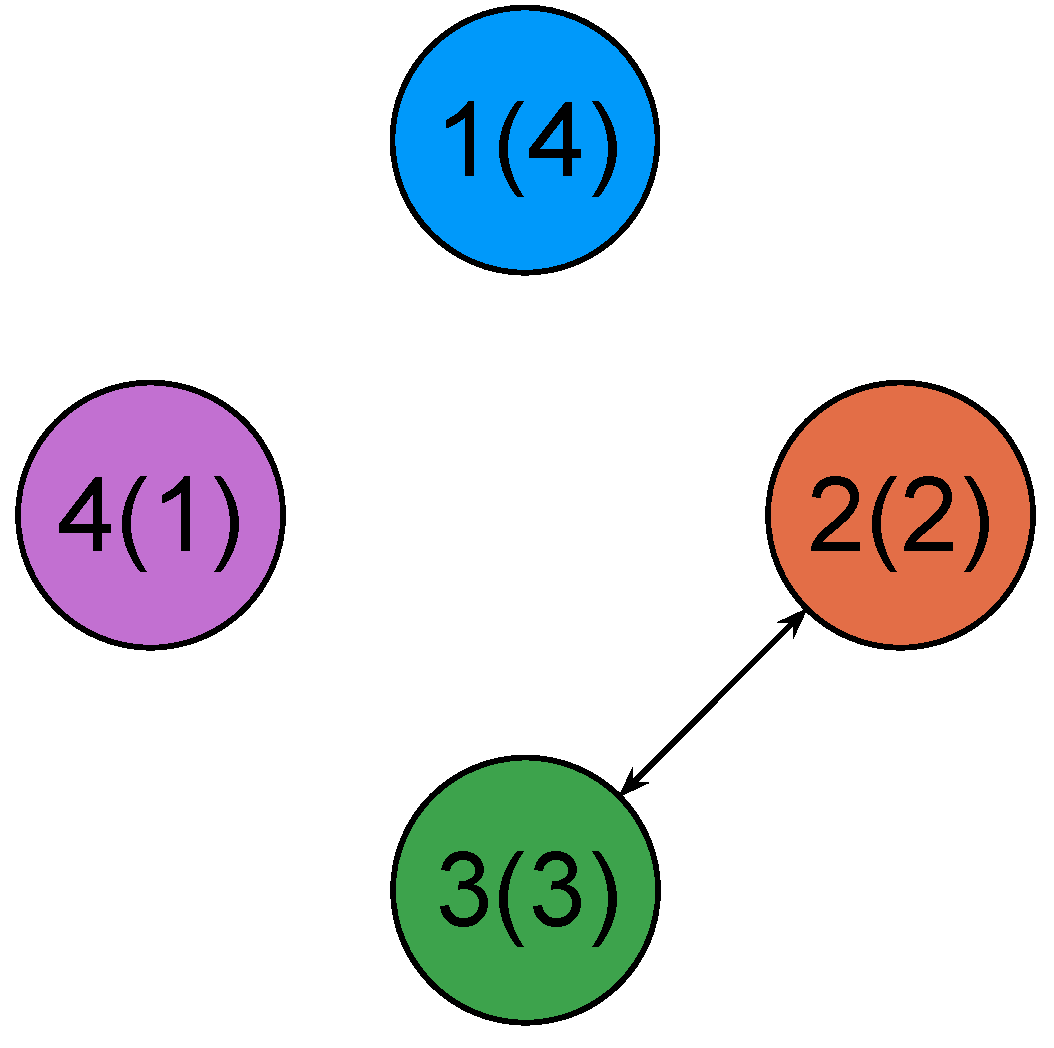
\includegraphics[width=0.39\textwidth]{../img/Communication_4_v3.pdf}
    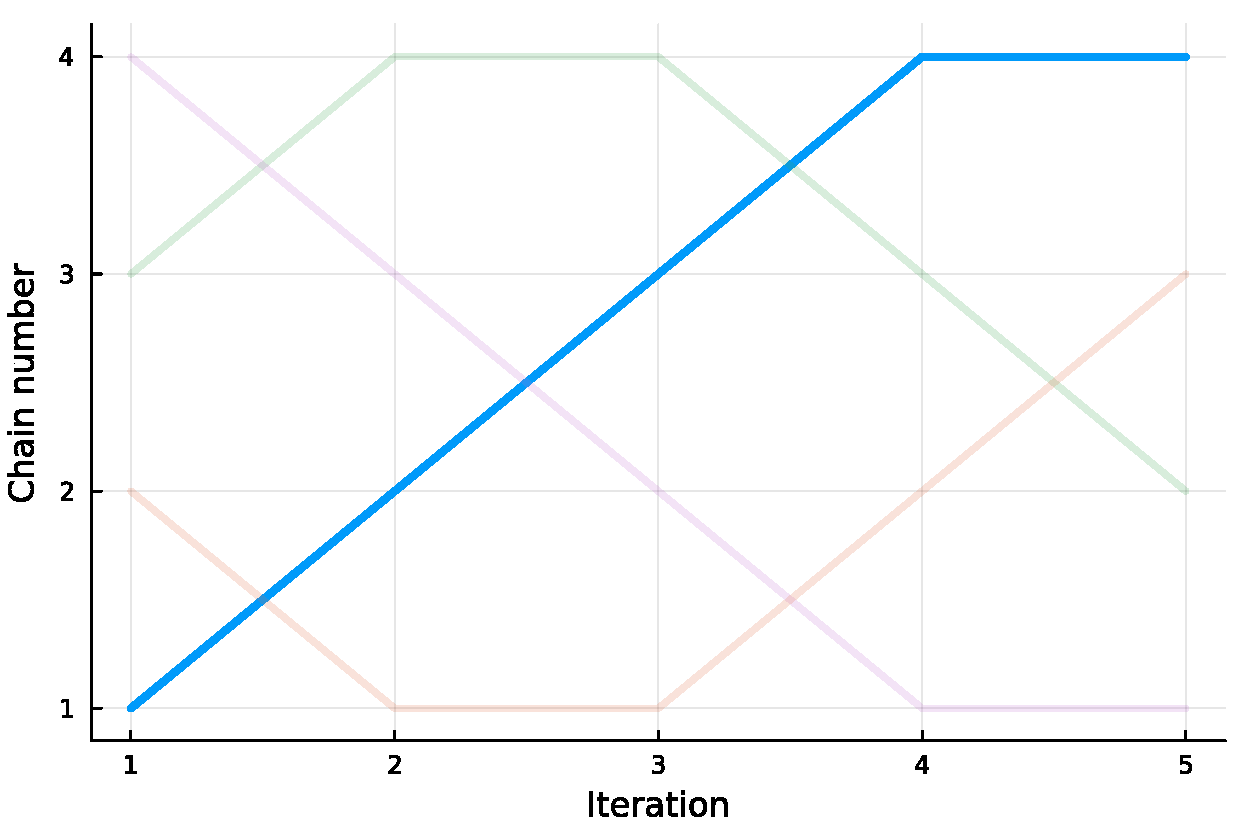
\includegraphics[width=0.59\textwidth]{../img/index_process_4.pdf}
  \end{minipage}
  \caption{
    A summary of communication between four machines with $N=4$ PT chains.
    Circles represent machines with the machine number in the center of the circle. 
    Different colours are also used for different machines.
    Numbers in parentheses represent the \texttt{chain} 
    that is currently being explored by that machine. 
    Arrows indicate communication occuring between machines to exchange \texttt{chain} 
    indices.
    To keep track of which chains are stored on which machine, we introduce the 
    \texttt{dist\_array} of type \texttt{PermutedDistributedArray}, described in 
    \cref{sec:permuted_dist_array}, which is of length $N$. 
    The $j$-th element of \texttt{dist\_array} at a given time step indicates which 
    machine number is storing \texttt{chain} index $j$.
    The bolded curve in the figures to the right indicate the trajectory of the first 
    \texttt{Replica} over the course of each of the communication steps.      
    \textbf{Top left:} the PT replicas are initialized and the first communication step 
    is proposed. At this time step, $\texttt{dist\_array} = [1,2,3,4]$.
    \textbf{Top right:} after the first successful communication step, we now have 
    $\texttt{dist\_array} = [2,1,4,3]$.
    \textbf{Bottom left:} The second communication step is completed and 
    $\texttt{dist\_array} = [2,4,1,3]$.
    \textbf{Bottom right:} The third communication step is completed and 
    $\texttt{dist\_array} = [4,2,3,1]$.}
  \label{fig:index_process}
\end{figure*}

\subsubsection{MPI implementation details}
We use the MPI.jl \cite{byrne2021mpi} package to support communication between machines. 
In  \cref{alg:distributed_PT}, the function \texttt{swap\_stat()} extracts the 
sufficient statistic required by each partner of a swap. The swap
sufficient statistic contains two elements:
(1) a uniformly distributed random number, and (2) the log of the ratio 
$\pi_c(x_t) / \pi_{c'}(x_t)$, up to a normalization constant which may 
depend on $c$ and $c'$ but not $x_t$.  
The function \texttt{transmit()} is used to exchange these statistics 
between the two partners of a proposed swap. In order to make an 
accept-reject decision, the two machines use the same uniform sample (using an arbitrary, fixed 
convention, namely the shared sufficient statistic's uniform from the lowest 
interacting chain index) to make a common swap decision (where the 
acceptance ratio is the sum of the two exchanged log ratios, (2)). 

 
In \cref{alg:distributed_PT} we also introduce the functions 
\texttt{permuted\_get()} and \texttt{permuted\_set!()}, which operate 
on a  \texttt{PermutedDistributedArray} as described  in \cref{sec:permuted_dist_array}.
Given the current machine's \texttt{dist\_array} and the 
\texttt{partner} chain with which it should communicate, 
\texttt{permuted\_get()} returns the machine number that holds the \texttt{partner} chain. 
Given the current machine's \texttt{dist\_array}, \texttt{chain} number, and machine number $j$,
\texttt{permuted\_set!()} updates the \texttt{PermutedDistributedArray} variables 
with the updated permutation.

\begin{algorithm}[t]
\footnotesize
	\begin{algorithmic}[1]
    \Require Initial state $x_0$, sequence of distributions $\{\pi_i\}_{i=1}^N$, 
      number of iterations $T$, machine number $j$
    \State $\texttt{chain} \gets j$ \Comment{current \texttt{chain} number}
    \State $\texttt{dist\_array}[j] \gets j$ \Comment{\texttt{chain} $j$ is on machine $j$}
		
    \For{$t$ {\bf in} 1, 2, \dots, $T$}
    
     \State $x_t \gets \texttt{local\_exploration}(\pi_\texttt{chain}, x_{t-1})$
    \State $c_t \gets \texttt{chain}$ 
    
		  \If{$\texttt{is\_even}(t) = \texttt{is\_even}(\texttt{chain})$} 
		    \State $\texttt{direction} \gets +1$
		  \Else
		    \State $\texttt{direction} \gets -1$
		  \EndIf
		  \State $\texttt{partner} \gets \texttt{chain} + \texttt{direction}$

     
      \If{$\texttt{partner} = 0$} 
        \State $\texttt{partner} \gets 1$ \Comment{Encode boundaries as self-interaction}
      \ElsIf{$\texttt{partner} = N + 1$}
        \State $\texttt{partner} \gets N$
      \EndIf
	    \State $\texttt{my\_stat} \gets \texttt{swap\_stat}(x_t, $\texttt{chain}, $\texttt{partner} )$  
      \State $\texttt{to\_machine} \gets  \texttt{permuted\_get}(\texttt{dist\_array}, \texttt{partner})$
      \State $\texttt{partner\_stat} \gets \texttt{transmit}(\texttt{my\_stat}, \texttt{to\_machine})$
      \If{$\text{swap\_accepted}(\texttt{my\_stat}, \texttt{partner\_stat})$}
        \State $\texttt{chain} \gets \texttt{partner\_chain}$
      \EndIf
      \State $\texttt{permuted\_set!}(\texttt{dist\_array}, \texttt{chain}, j)$ 
		\EndFor
    \State \Return $\{(x_t, c_t)\}_{t=1}^T$
	\end{algorithmic}
  \caption{Distributed PT on machine $j$ (one replica per machine)}
  \label{alg:distributed_PT}
\end{algorithm}

\subsubsection{Load balancing}
\label{sec:relax}

So far we have assumed, for pedagogy, that the number of 
machines $M$ is equal to the number of chains $N$.
This restriction is not present in Pigeons, so we now describe how 
the code base generalizes \cref{alg:distributed_PT}. 
First, the $N$ replicas are shared between the $M$ machines so that 
each machine contains either $\lceil N/M \rceil$ or $\lfloor N/M \rfloor$ 
replicas. Each machine's replicas are called the local replicas. 
The allocation of replicas to machine is fixed over the whole execution of the 
algorithm and maintained using the \texttt{LoadBalance} struct. 
Second, the code performing local exploration is enclosed in a 
loop over the local replicas, and if the option ``\texttt{multithreaded = true}'' 
is used in the \texttt{pigeons(...)} call, the exploration loop is performed in a 
\texttt{@threads for} loop. 
Finally, the functions used in the communication, 
\texttt{permuted\_get}, \texttt{permuted\_set!}, \texttt{transmit}, etc., 
are vectorized to accommodate that \texttt{chain} and 
\texttt{partner} are no longer integers but rather sets of integers. 
In particular, the permuted distributed array is designed so that each 
machine is responsible for tracking machine allocations for 
$\lceil N/M \rceil$ or $\lfloor N/M \rfloor$ chains instead of a single one.


\subsection{Weak scaling of PT}

We study the weak scaling properties of Pigeons' implementation of PT.
In this setup, we consider a varying problem size proportional to the number of processes used. 
The number of chains is our definition of the problem size; 
this is in line with previous heuristics that establish that the problem 
difficulty is generally proportional to the optimal number of chains in PT \cite{syed2021nrpt}.
In particular, we consider a multivariate normal target distribution 
and vary the dimension $d \in \cbra{2^1, 2^2, \ldots, 2^{12}}$ for the distributed setup and 
$d \in \cbra{2^1, 2^2, \ldots, 2^{10}}$ for the parallel (shared memory) setup. 
The number of chains is set to $\ceil{\sqrt{d}}$ according to PT tuning suggestions \cite{syed2021nrpt} 
and for the distributed and parallel settings we set the number of processes or threads equal 
to the number of chains.
Within each chain we use the autoMALA sampler \cite{biron2024automala}, which is a 
gradient-based sampler with automatic step size selection in the Metropolis-adjusted Langevin algorithm.
Ten different seeds are used in order to obtain approximate 95\% confidence intervals of 
the speedup.


The weak scaling results for both the distributed memory parallelism (DMP) and 
shared memory parallelism (SMP) settings are presented in \cref{fig:PT_scaling}. 
We see that we obtain an approximately linear speedup as we increase the number of processes. 

\begin{figure*}[t]
    \centering
    \begin{minipage}{0.4\textwidth}
      \centering
      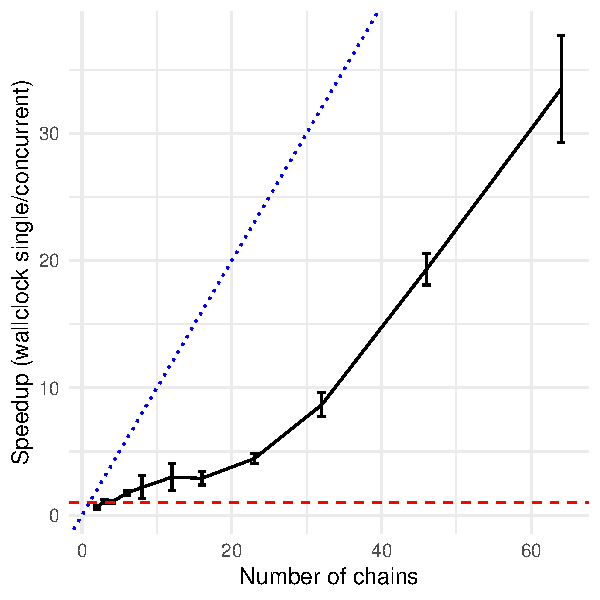
\includegraphics[width=\textwidth]{../img/speedup_distributed.pdf}
    \end{minipage}
    \begin{minipage}{0.4\textwidth}
      \centering
      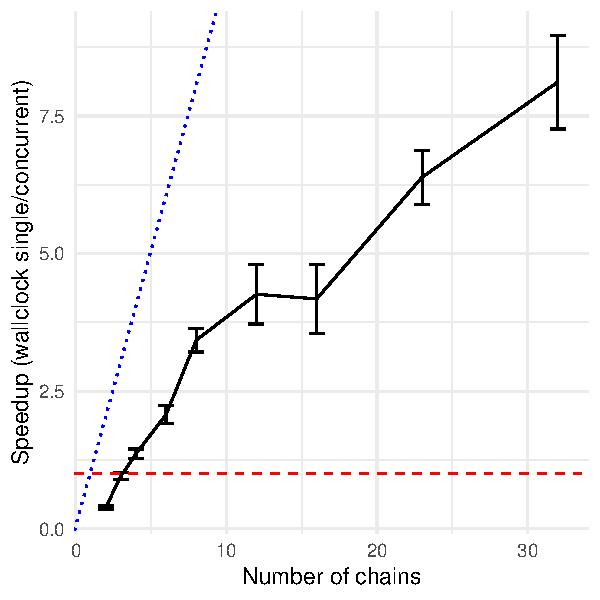
\includegraphics[width=\textwidth]{../img/speedup_parallel.pdf}
    \end{minipage}
    \caption{
        Weak scaling results for PT in both the distributed (MPI, {\bf left}) 
        and parallel (Julia threads, {\bf right}) settings 
        with approximate 95\% confidence intervals for the speedup relative to single-thread execution.   
        The blue dotted line represents a hypothetical speedup equal to the 
        number of processes/threads. 
        The red dashed line indicates a speedup of one for reference.
    }
    \label{fig:PT_scaling}
\end{figure*}


\subsection{Relevance of DMP versus SMP}

We emphasize again that Pigeons supports both shared memory 
parallelism (SMP) and distributed memory parallelism (DMP). However, in certain cases, it 
might be useful to run parallel tempering with  many chains or 
to run several instances of parallel tempering at once. In such cases, 
the DMP setup is the most natural if the requested number of chains is very large. 
Another notable example of the benefit of DMP is for the multi-GPU use case. 
For instance, in some situations the likelihood evaluation of a single chain may 
require its own GPU (e.g., if one is running a Fast Fourier Transform on a GPU). 
Additionally, DMP can be useful when the user's code is not thread safe. 
In such cases, concurrency can still be achieved via DMP.
Our implementation in Pigeons ensures that the 
communication cost in the DMP setup is minimal. In most cases, the 
communication cost is negligible compared to other computations performed on each process. 

